%% ------------------------------------------------------------------------- %%
\chapter{Desenvolvimento}
\label{cap:desenvolvimento}

A proposta inicial do projeto consiste em rodar um experimento em pequena escala. Extraímos informações de um número pequeno de currículos Lattes, com interesse nas informações básicas dos pesquisadores do Departamento de Computação do Instituto de Matemática e Estatística da USP. Dados como nome, área de atuação, publicações, coautores, local de trabalho ou residência, e data em que começou a trabalhar no instituto.

Com base nessas informações, modelamos uma ontologia utilizando OWL através do software Protégé. Esse software facilita a construção, edição, e consulta a ontologias.

Essa ontologia tem por finalidade organizar o conhecimento a respeito de pesquisadores e sua origem acadêmica, suas publicações, e os relacionamentos entre essas entidades. Com isso, é possível acessar informações estruturadas acerca da produção bibliográfica e científica dos docentes e alunos do instituto, servindo de base para esse experimento.

%TODO falar do FOAF

A ontologia possui a seguinte estrutura (TBOX):

%TODO conferir ontologia

\begin{alltt}
Class: Grupo \( \equiv \) foaf:Group
SubClassOf: Agent
Descrição: \emph{Classe que é pai de diferentes outras classes que definem grupos de pessoas.}
Relações:
  membros \( \equiv \) member

Class: Grupo_de_Pesquisa
SubClassOf: Grupo
Descrição: \emph{Classe dos grupos de pesquisa científica.}

Class: Organização \( \equiv \) foaf:Organization
SubClassOf: Agent
Descrição: \emph{Define uma organização, que pode ser uma Universidade, por
exemplo.}
Relações:
  faz_parte \( \equiv \) sub_organizacao: \emph{Uma \textbf{Organização}
pode fazer parte de outra \textbf{Organização}, por exemplo: o
Instituto de Física faz parte da USP.}
  possui \( \equiv \) super_organizacao: \emph{Uma \textbf{Organização} pode
possuir outra \textbf{Organização}, por exemplo: A USP possui o
Instituto de Matemática e Estatística.}

Class: Universidade
SubClassOf: Organização
Descrição: \emph{Classe das universidades e instituições
de ensino.}

Class:Instituto
SubClassOf: Organização
Descrição: \emph{Classe dos institutos de ensino e pesquisa e faculdades.}

Class: Departamento
SubClassOf: Organização
Descrição: \emph{Classe dos departamentos ligados a institutos de pesquisa ou
faculdades.}

Class: Revista
SubClassOf: Organização
Descrição: \emph{Classe das revistas científicas que publicam artigos.}
Relações:
  publicou: \emph{Uma \textbf{Revista} pode publicar um \textbf{Artigo}.
É o inverso da relação \textbf{publicado_em}.}

Class: Pessoa \( \equiv \) foaf:Person
SubClassOf: Agent
Descrição: \emph{Classe-pai dos tipos de pessoa.}
Relações:
  cursou: \emph{Uma \textbf{Pessoa} pode cursar algum \textbf{Curso}.}
  estudou_em: \emph{Uma \textbf{Pessoa} pode ter estudado em alguma
\textbf{Universidade, Instituto, Faculdade}.}
  membro_de: \emph{uma \textbf{Pessoa} pode ser membro de um  \textbf{Grupo}.
É o inverso da relação \textbf{membro}.}
  autor: \emph{Uma \textbf{Pessoa} pode ser autora de um  \textbf{Documento}.
É o inverso da relação \textbf{tem_autores}.}
  trabalhou_em: \emph{uma \textbf{Pessoa} pode trabalhar ou ter trabalhado
em uma \textbf{Organização}.}

Class: Aluno
SubClassOf: Pessoa
Descrição: \emph{Classe dos indivíduos que são alunos de algum curso.}
Relações:
  tem_orientador: \emph{Um \textbf{Aluno} pode ser orientado por um
\textbf{Professor} ou outro pesquisador.}

Class: Professor
SubClassOf: Pessoa
Descrição: \emph{Classe dos professores.}
Relações:
  orienta: \emph{Um \textbf{Professor} pode orientar um
\textbf{Aluno}. É o inverso da relação \textbf{tem_orientador}.}
  tem_orientador: \emph{Um \textbf{Professor} pode ser orientado por
um outro \textbf{Professor}, mesmo que no passado.}

Class: Curso
SubClassOf: Thing
Descrição: \emph{Classe dos cursos de graduação e pós-graduação.}
Relações:
  cursado_por: \emph{Um \textbf{Curso} pode ser cursado por \textbf{Pessoas}.}
  tipo_de_curso: \emph{Um \textbf{Curso} pode ser de Pós-Graduação ou
Graduação.}
  oferecido_por: \emph{Pode ser oferecido por uma instituição.}

Class: Graduação
SubClassOf: Tipo de Curso
Descrição: \emph{Classe dos cursos de graduação.}

Class: Pós Graduação
SubClassOf: Tipo de Curso
Descrição: \emph{Classe dos cursos de pós-graduação.}

Class: Documento \( \equiv \) foaf:Document
SubClassOf: Thing
Descrição: \emph{Classe dos documentos produzidos por alunos,
professores e pesquisadores.}
Relações:
  tem_autores: \emph{Um documento possui um ou mais autores do tipo
\textbf{Pessoa}. Essa propriedade é importante pois indica uma relação de \textbf{coautoria}.}

Class: Publicacao
SubClassOf: Documento
Descrição: \emph{Classe dos artigos científicos e outras publicações de
revistas, simpósios e outros eventos.}
Relações:
  publicado_em: \emph{Um \textbf{Publicacao} pode ser publicado em
uma \textbf{Revista} ou um \textbf{Evento}.}

Class: Tese
SubClassOf: Documento
Descrição: \emph{Classe-pai das Teses científicas de doutorado e dissertações de mestrado.}

Class: Eventos
SubClassOf: Thing
Descrição: \emph{Classe-pai dos eventos científicos, conferências, e simpósios.}
Relações:
  publicou: \emph{Um \textbf{Evento} pode ter publicações de \textbf{Artigos}.}

Class: foaf:Spatial Thing
Descricão: \emph{Classe dos indivíduos que possuem alguma
localização geográfica. \textbf{Evento} é uma delas.}

Classe: Local
SubClassOf: Thing
Descrição: \emph{Classe dos locais geográficos; são localizações.}
Relações:
  localizado \( \equiv \) foaf:based near \emph{Relaciona \textbf{Organização} ou \textbf{Evento} com um local
geográfico.}

Class: País
SubClassOf: Local

Class: Continente
SubClassOf: Local

\end{alltt}

A ontologia foi populada com as informações dos currículos lattes, e algumas consultas também farão parte da definição da ontologia. Essas consultas são escritas na linguagem SPARQL. Duas consultas que nos interessam agora respondem às seguintes perguntas:

\begin{itemize}
    \item Qual a área de pesquisa de um pesquisador?
    \item Quem são os pesquisadores que ele orientou?
    \item Há quantos anos um dado pesquisador trabalha em uma instituição?
\end{itemize}

A primeira questão de competência é extraída diretamente do currículo lattes. A segunda questão pode ser respondida através da relação \textit{orienta} das instâncias da classe \textit{Professor}. Um professor terá uma lista de orientandos, que também são pesquisadores.

Já a questão a respeito dos anos de trabalho em uma dada instituição

%TODO Conhecimento Prévio

O conhecimento prévio, que chamaremos de $BK$, será extraído da ontologia através das consultas SPARQL, e estruturado em uma tabela da seguinte forma: seja $P$ o conjunto de pesquisadores presentes na ontologia. Cada linha dessa tabela resultante corresponde à um elemento do conjunto $Q = \{ (a, b) | a \in P \text{ e } b \in P \text{ e } a \neq b \}$, e cada coluna indica algum atributo de $a$ ou $b$ extraído da ontologia ou alguma das diversas possíveis relações entre um desses pares de pesquisadores. A coluna assume o valor $1$ se a relação existir, e $0$ se não existir.

Como exemplo, temos $P = \{ p_1, p_2, p_3 \}$ e o conjunto de relações $R = \{ orienta, coautor \}$, e sabemos que $p_1$ \texttt{orienta} $p_2$, pois $p_1$ foi orientador de $p_2$ em seu doutorado. E também sabemos que $p_1$ \texttt{coautor} $p_2$ e $p_1$ \texttt{coautor} $p_3$ e $p_2$ \texttt{coautor} $p_3$, pois os três publicaram um artigo juntos. A matriz resultante será:

\begin{table}[h!]
    \centering
    \begin{tabular}{|c|c|c|}
     \hline
      & orienta & coautor \\
     \hline\hline
     $(p_1, p_2)$ & 1 & 1  \\
     \hline
     $(p_1, p_3)$ & 0 & 1  \\
     \hline
     $(p_2, p_3)$ & 0 & 1  \\
     \hline
    \end{tabular}
    \caption{Matriz de relacionamentos entre pesquisadores}
    \label{matriz-relacoes}
\end{table}

Durante o treinamento do modelo de predição, o conjunto de treinamento conterá a coluna coautor, que define se esse exemplo pertence ou não à categoria "coautor". Durante os testes, o modelo deverá prever se existe ou não uma relação de coautoria a partir das outras propriedades contidas nas demais colunas, classificando cada um dos exemplos em uma classe $1$ (existe relação de coautoria), ou $-1$ (não existe relação de coautoria). A classificação será validada através da coluna coautor, e será possível medir a eficácia do método de predição.

%Enriquecimento

O conjunto de informações geradas através do grafo com atributos será enriquecido com as informações extraídas do conjunto $BK$. Chamamos aqui de enriquecimento a adição de novos atributos aos elementos do conjunto $P$. Cada pesquisador possui um conjunto de atributos relevantes, e esse conjunto será expandido com as informações do conjunto $BK$.

%??

%colocar o diagrama
%TESTES

Vamos testar inicialmente dois modelos de predição: Máquinas de Vetores de Suporte e Árvores de Decisão.
SMVs são importantes porque...
Árvores de decisão são...

O modelo receberá como estrada um conjunto de treinamento onde cada linha corresponde a um elemento do conjunto $Q$, sendo cada coluna uma propriedade de um dos pesquisadores, um atributo ou uma relação extraídos de $BK$.

Um dos modelos será treinado com dados apenas dos pesquisadores (conjunto inicial sem o enriquecimento), e será testado, tendo sua eficácia será analisada.

Outro modelo será treinado apenas com o conjunto enriquecido com as informações de $BRK$, será testado, e sua eficácia será analisada.

Por fim, faremos a comparação da eficácia entre ambos os modelos, verificando se há melhoria na eficácia quando utilizamos conhecimento prévio.

Também é de interesse avaliar se os atributos adicionais extraídos de $BK$ são relevantes. O modelo SVM é %???


O ambiente de testes recebe um conjunto de currículos e um arquivo OWL correspondente à estrutura da ontologia, porém sem nenhuma instância.

(1)O programa será responsável por ler os currículos e popular a ontologia com esses dados.

(2) Um dos módulos será responsável por construir o grafo com atributos e extrair o conjunto de dados sobre pesquisadores e o vetor de características. %pegar de cervantes
%como? quais atributos? como é o grafo?

%TODO explicar diagrama
\begin{figure}[!h]
  \centering
  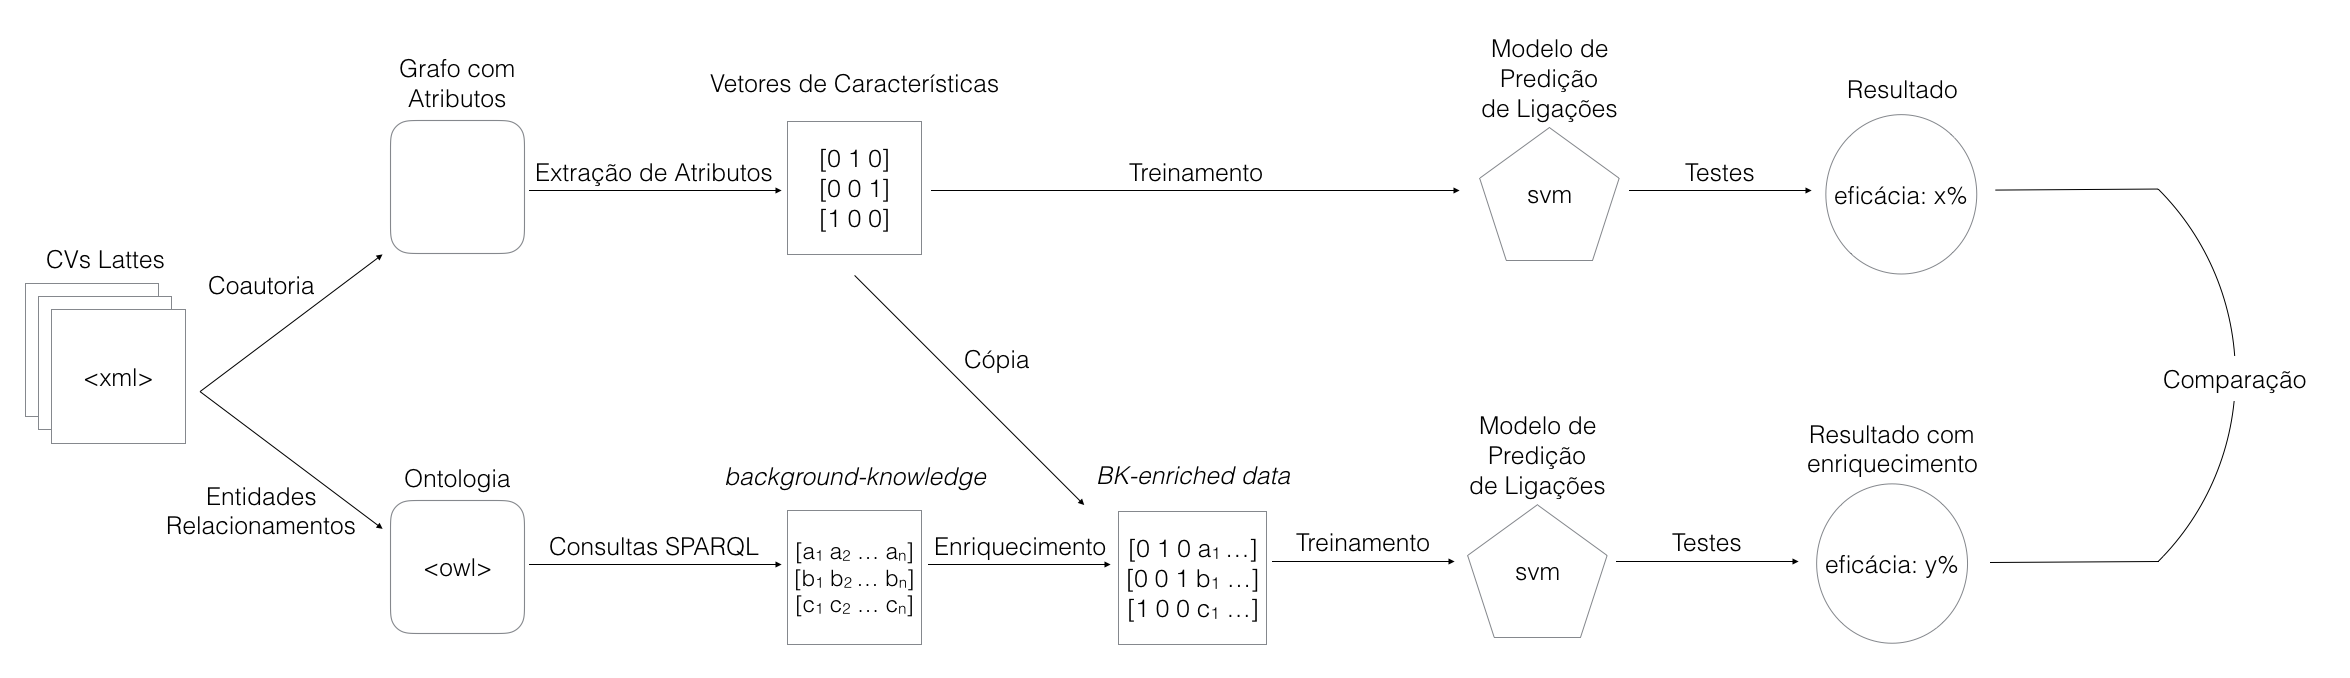
\includegraphics[width=.99\textwidth]{diagrama-menor}
  \caption{Diagrama de execução do experimento}
  \label{fig:diagrama-experimento}
\end{figure}

(3) Após isso, deve rodar consultas SPARQL e extrair o conhecimento prévio $BK$.

(4) Com esses arquivos gerados, o programa vai ler os dados extraídos por (2) e enriquecer o conjunto $BK$ com o vetor de características.

(5) O programa deve instanciar um modelo de predição e triná-lo com as informações apenas dos vetores de características
(6) O programa deve instanciar outro modelo de predição e treinálo com as informações enriquecidas em $BK$

(7) O programa deve rodar os testes de ambos os modelos, calculando sua eficácia, e deve gerar um relatório comparando ambas as metodologias.

(8) O programa deve ainda avaliar se as características contidas nos atributos de $BK$ são relevantes.



%1. Estudar o domínio e modelar uma Ontologia.
%2. Modelar as consultas à ontologia que servirão para enriquecer o modelo de predição.
%3. Construir um modelo de predição de ligações baseado nos trabalhos da literatura, fazendo experimentos com diferentes técnicas de aprendizado supervisionado.
%4. Propor e implementar um algoritmo de extração de conhecimento da ontologia e enriquecimento do modelo de predição.
%5. Montar ambiente de testes e elaborar alguns testes de comparação.
